\newpage
\section{Soal 3: Seleksi Fitur Fisikokimia Wine dengan Genetic Algorithm}

Dataset yang dipakai adalah D4 Wine Quality (red wine) dengan 1.599 sampel dan 11 fitur fisikokimia. GA dijalankan dengan \texttt{pygad}.

\subsection{Business Understanding}
Produsen wine ingin tahu kandungan kimia apa yang paling membedakan wine berkualitas tinggi dari yang rendah, supaya uji laboratorium cukup difokuskan ke beberapa parameter. Mirip dokter yang memeriksa beberapa tanda vital yang paling informatif, tidak semua organ.

Ada tiga hal yang ingin dijawab: subset fitur mana yang memaksimalkan skor $J(S)$, apakah GA memberi jawaban yang sama di seed berbeda, dan apakah fitur yang terpilih memang punya distribusi berbeda antar-kelompok. Kriteria kesuksesannya saya tetapkan sebelum eksperimen:

\begin{tabularx}{\textwidth}{@{}LL@{}}
\toprule
\textbf{Kriteria kesuksesan} & \textbf{Ambang} \\
\midrule
GA mencapai optimum hasil \emph{brute force} ($2^{11} = 2048$ subset) & selisih $J$ = 0 \\
Konsistensi antar-run (5 seed) & $\geq$ 4 dari 5 run menghasilkan subset sama \\
Fitur terpilih berbeda signifikan antar-kelompok & Mann-Whitney $p < 0.05$ \\
Subset tetap memisahkan kelas di data \emph{hold-out} & balanced accuracy $\geq 0.75$ \\
\bottomrule
\end{tabularx}

\subsection{Data Understanding dan Data Preparation}
Datanya tidak punya missing value, tetapi ada 240 baris duplikat (sekitar 15\%). Outlier paling banyak muncul di \textit{residual sugar} (155) dan \textit{chlorides} (112), dan keduanya miring ke kanan. Skor \textit{quality} menumpuk di 5 dan 6. Dari korelasi, \textit{alcohol} paling berhubungan positif dengan kualitas dan \textit{volatile acidity} paling negatif.

Duplikat saya buang, karena baris kembar terhitung dua kali di mean dan std, dan salinannya bisa jatuh ke data latih dan \emph{hold-out} sekaligus. Sesuai soal, kelompok H berisi $q \geq 7$, kelompok L berisi $q \leq 5$, dan $q = 6$ dibuang. Outlier tetap dipakai karena merupakan hasil uji lab yang sah. Setelah itu tersisa 824 sampel (H = 184, L = 640).

Data lalu dibagi 80:20 secara berstrata. $J(S)$ dan GA hanya melihat data latih (659 sampel), sedangkan 165 sampel \emph{hold-out} baru dipakai di akhir untuk memeriksa apakah subset terpilih memang informatif. Scaling tidak diperlukan, karena $J(S)$ sudah membagi selisih mean dengan simpangan baku sehingga satuannya hilang.

\fig{soal_03_1.png}{0.9}{Distribusi skor \textit{quality} dan korelasi tiap fitur dengan \textit{quality}.}

\jawab{Jawaban 3a: Makna komponen $J(S)$, penalti, dan kromosom kosong}
\[ J(S) = \sum_{j \in S} \frac{|\mu_{H,j} - \mu_{L,j}|}{\sigma_{H,j} + \sigma_{L,j} + \varepsilon} - 0.10\,|S| \]

\begin{tabularx}{\textwidth}{@{}lL@{}}
\toprule
\textbf{Komponen} & \textbf{Makna} \\
\midrule
$|\mu_{H,j} - \mu_{L,j}|$ & Jarak rata-rata fitur $j$ antara wine bagus dan wine jelek. Makin jauh, makin membedakan. \\
$\sigma_{H,j} + \sigma_{L,j}$ & Sebaran nilai di tiap kelompok. Selisih rata-rata 1 tidak berarti apa-apa kalau data menyebar $\pm$10, tetapi sangat berarti kalau sebarannya hanya $\pm$0.1. Pembagian ini membuat skor tanpa satuan, mirip \emph{signal-to-noise ratio}. \\
$\varepsilon$ & Angka sangat kecil ($10^{-9}$) supaya tidak terjadi pembagian dengan nol. \\
$-0.10|S|$ & Penalti 0.10 untuk setiap fitur yang dipakai. \\
\bottomrule
\end{tabularx}

Penalti diperlukan karena setiap suku pemisahan bernilai $\geq 0$. Tanpa penalti, menambah fitur tidak pernah menurunkan $J$, sehingga jawaban terbaik selalu ``pakai semua fitur''. Dengan penalti 0.10, sebuah fitur harus membayar semacam tiket masuk: ia hanya layak dipakai kalau skor pemisahannya lebih dari 0.10.

Kromosom kosong (semua gen 0) secara rumus menghasilkan $J = 0$, padahal tanpa fitur tidak ada yang bisa dipisahkan. Saya memberinya fitness $-10$. Subset valid tidak mungkin bernilai di bawah $-0.10 \times 11 = -1.1$ karena skor pemisahan selalu $\geq 0$, jadi kromosom kosong selalu kalah dan cepat hilang dari populasi.

Satu hal yang membantu pemeriksaan: $J(S)$ adalah jumlah skor per fitur, dan fitur-fitur itu tidak saling mempengaruhi. Optimum sebenarnya bisa dicari dengan mencoba semua 2048 subset, dan hasilnya ($J = 2.4708$ dengan 8 fitur) saya pakai sebagai kunci jawaban untuk menilai GA.

\jawab{Jawaban 3b: Desain GA dan pengaruh \emph{mutation rate}}
\begin{tabularx}{\textwidth}{@{}llL@{}}
\toprule
\textbf{Komponen} & \textbf{Pilihan} & \textbf{Alasan} \\
\midrule
Representasi & biner, 11 gen & satu gen = saklar satu fitur \\
Populasi / generasi & 30 / 50 & ruang solusi hanya 2048, jadi 30 individu sudah beragam \\
Jumlah orang tua & 10 per generasi & sepertiga populasi, cukup beragam tanpa memberi kesempatan pada individu lemah \\
Seleksi & \emph{tournament}, $k = 3$ & tekanan seleksi sedang, populasi tidak terlalu cepat seragam \\
Crossover & \emph{uniform}, $p = 0.9$ & urutan fitur tidak bermakna, jadi tiap gen diwarisi acak \\
Mutasi & \emph{random} pada \{0,1\}, $p = 0.10$ & peluang gen benar-benar terbalik sekitar 0.05 \\
Elitisme & 2 individu & solusi terbaik tidak pernah hilang \\
\bottomrule
\end{tabularx}

Mutasi bisa dibayangkan sebagai rasa penasaran populasi. Untuk melihat pengaruhnya, GA saya jalankan dengan lima nilai \emph{mutation rate}, masing-masing dengan 5 seed:

\begin{adjustbox}{max width=\textwidth}\begin{tabular}{@{}lcccc@{}}
\toprule
\textbf{Mutation rate} & \textbf{Run capai optimum} & \textbf{Rata-rata generasi capai} & \textbf{Mean fitness akhir} & \textbf{Keragaman akhir} \\
\midrule
0.01 & 5/5 & 5.2 & 2.438 & 0.33 \\
0.05 & 5/5 & 4.4 & 2.335 & 1.23 \\
0.10 & 5/5 & 4.4 & 2.135 & 3.04 \\
0.30 & 5/5 & 8.2 & 1.597 & 5.15 \\
0.60 & \bad{2/5} & 6.5 & 1.204 & 5.52 \\
\bottomrule
\end{tabular}\end{adjustbox}

Dengan 0.01, keragaman akhir tinggal 0.33 bit, artinya hampir semua individu sudah kembar dan populasi rawan konvergensi prematur. Di soal ini hasilnya masih aman hanya karena ruang solusinya kecil. Nilai 0.05 sampai 0.10 menemukan optimum paling cepat (rata-rata generasi ke-4,4) sambil tetap menjaga populasi beragam, jadi 0.10 saya pakai untuk GA utama. Di 0.60, GA hampir berubah menjadi \emph{random search} dan hanya 2 dari 5 run yang sampai ke optimum.

\jawab{Jawaban 3c: Hasil 5 run GA}
Kelima run (seed 47 sampai 51) menghasilkan subset yang persis sama: 8 fitur dengan $J = 2.4708$, identik dengan optimum \emph{brute force}. Fiturnya adalah \emph{alcohol, volatile acidity, sulphates, citric acid, density, total sulfur dioxide, chlorides,} dan \emph{fixed acidity}.

\begin{figure}[H]\centering
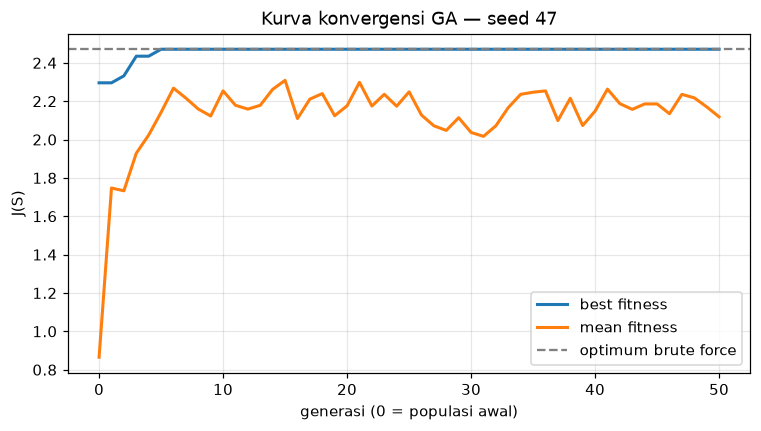
\includegraphics[width=0.49\textwidth]{figures/soal_03_3.png}\hfill
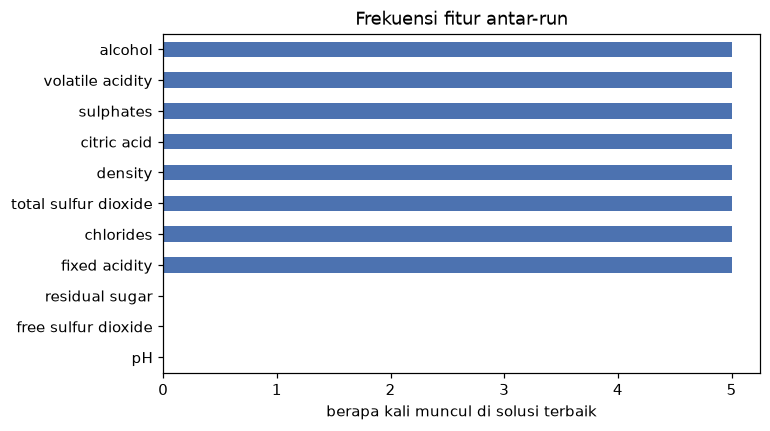
\includegraphics[width=0.46\textwidth]{figures/soal_03_4.png}
\caption{Kiri: kurva konvergensi GA seed 47; \emph{best fitness} mencapai optimum di generasi ke-5. Kanan: frekuensi fitur pada solusi terbaik dari 5 run.}
\end{figure}

\begin{adjustbox}{max width=\textwidth}\begin{tabular}{@{}lcc|lcc@{}}
\toprule
\textbf{Fitur} & \textbf{Frek.} & \textbf{Skor} & \textbf{Fitur} & \textbf{Frek.} & \textbf{Skor} \\
\midrule
alcohol & 5 & 0.964 & total sulfur dioxide & 5 & 0.239 \\
volatile acidity & 5 & 0.575 & chlorides & 5 & 0.220 \\
sulphates & 5 & 0.405 & fixed acidity & 5 & 0.185 \\
citric acid & 5 & 0.376 & residual sugar & 0 & 0.081 \\
density & 5 & 0.307 & free sulfur dioxide & 0 & 0.080 \\
 & & & pH & 0 & 0.064 \\
\bottomrule
\end{tabular}\end{adjustbox}

Tiga fitur tidak pernah terpilih karena skornya 0.06-0.08, di bawah penalti 0.10. GA sangat stabil karena $J(S)$ bisa dipecah per fitur dan ruang solusinya kecil, jadi tidak ada optimum lokal yang menjebak. Fitur yang paling tipis lolosnya adalah \emph{fixed acidity}, hanya 0.085 di atas penalti.

Stabil terhadap seed belum tentu stabil terhadap data. Kalau $J$ dihitung dari seluruh data tanpa split, \emph{free sulfur dioxide} ikut lolos dengan skor 0.127 dan hasilnya menjadi 9 fitur, padahal di data latih skornya hanya 0.080. Fitur ini berada tepat di sekitar ambang. Split tetap saya pakai supaya pemilihan fitur tidak melihat data \emph{hold-out}, sesuai petunjuk UTS no.~4.

\jawab{Jawaban 3d: Apakah fitur terpilih benar-benar terpisah?}
Skor $J$ hanya memakai mean dan std, dan mean mudah terseret outlier. Karena itu pemisahannya saya uji lagi dengan uji peringkat Mann-Whitney (tahan outlier), Kolmogorov-Smirnov (KS), dan AUC satu fitur.

\begin{adjustbox}{max width=\textwidth}\begin{tabular}{@{}lcccccc@{}}
\toprule
\textbf{Fitur} & \textbf{Terpilih} & \textbf{Median H} & \textbf{Median L} & \textbf{AUC} & \textbf{KS} & \textbf{$p$ Mann-Whitney} \\
\midrule
alcohol & ya & 11.70 & 9.70 & 0.912 & 0.691 & $1.4\times10^{-52}$ \\
volatile acidity & ya & 0.38 & 0.59 & 0.803 & 0.492 & $3.6\times10^{-29}$ \\
sulphates & ya & 0.74 & 0.58 & 0.795 & 0.521 & $8.0\times10^{-28}$ \\
fixed acidity & ya & 8.70 & 7.80 & 0.619 & 0.224 & $1.1\times10^{-5}$ \\
free sulfur dioxide & tidak & 12.0 & 15.0 & 0.560 & 0.124 & 0.027 \\
pH & tidak & 3.27 & 3.31 & 0.550 & 0.119 & 0.065 \\
\bottomrule
\end{tabular}\end{adjustbox}

\fig{soal_03_5.png}{1.0}{Distribusi H vs L: dua fitur terkuat, fitur terpilih terlemah (\emph{fixed acidity}), dan fitur tidak terpilih (pH).}

Fitur terkuat memang terpisah dengan jelas. AUC 0.91 pada \emph{alcohol} berarti 91\% kemungkinan wine bagus punya alkohol lebih tinggi dari wine jelek, dan histogram kedua kelompok hampir tidak bertumpuk. Kedelapan fitur terpilih signifikan ($p \leq 1.1\times10^{-5}$), tetapi kekuatannya berbeda: distribusi \emph{fixed acidity} (KS 0.22) masih banyak bertumpuk. Dengan ratusan sampel, perbedaan kecil pun bisa signifikan, jadi signifikan belum tentu kuat secara praktis. Fitur yang tidak dipilih memang lemah; pH bahkan tidak signifikan dan histogram H dan L-nya hampir identik.

Kelemahan $J(S)$ ada pada redundansi. \emph{Fixed acidity} berkorelasi 0.67 dengan \emph{citric acid} dan 0.63 dengan \emph{density}, sedangkan \emph{density} berkorelasi $-0.48$ dengan \emph{alcohol}. Di data \emph{hold-out}, logistic regression dengan 8 fitur GA mendapat balanced accuracy 0.826, dengan semua 11 fitur 0.822, dan dengan 3 fitur teratas saja 0.802. Sebagian fitur ternyata membawa informasi yang sama.

Jadi fitur yang sering dipilih memang memisahkan distribusi secara nyata, terutama \emph{alcohol}, \emph{volatile acidity}, dan \emph{sulphates}. Untuk perbaikan, fitness bisa diberi penalti korelasi antar-fitur terpilih seperti pada mRMR.

\subsection{Interpretasi Hasil}
Logistic regression dengan 8 fitur hasil GA, diuji pada data \emph{hold-out}, mencapai accuracy 0.848 dan balanced accuracy 0.826. Dari 37 wine berkualitas tinggi, 29 terdeteksi (recall 0.784). Kesalahan terbanyak berasal dari 17 wine biasa yang terlihat bagus, misalnya beralkohol tinggi tetapi berkualitas rendah.

\begin{adjustbox}{max width=\textwidth}\begin{tabular}{@{}llll@{}}
\toprule
\textbf{Kriteria} & \textbf{Target} & \textbf{Hasil} & \textbf{Status} \\
\midrule
GA = optimum \emph{brute force} & selisih 0 & $J = 2.4708$ (5 run) & \ok{tercapai} \\
Konsistensi antar-run & $\geq 4/5$ & 5/5 & \ok{tercapai} \\
Fitur terpilih signifikan & $p < 0.05$ & 8/8 & \ok{tercapai} \\
Separasi \emph{hold-out} & $\geq 0.75$ & 0.826 & \ok{tercapai} \\
\bottomrule
\end{tabular}\end{adjustbox}

GA biner menemukan subset optimal 8 dari 11 fitur dan memberi jawaban yang sama di semua seed, terutama karena $J(S)$ bisa dipecah per fitur dan ruang solusinya kecil. \emph{Mutation rate} 0.05 sampai 0.10 paling efisien. Kalau anggaran uji lab terbatas, \emph{alcohol}, \emph{volatile acidity}, dan \emph{sulphates} saja sudah memberi balanced accuracy 0.80.
